\\documentclass\[12pt,a4paper\]{ctexart}

% 宏包顺序：正文宏包在前，hyperref放最后
\\usepackage{amsmath,amssymb}
\\usepackage{graphicx}
\\usepackage{booktabs}
\\usepackage{geometry}
\\usepackage{float}
\\usepackage{setspace}
\\usepackage{ctex} % 中文支持

% 页面边距
\\geometry{
    left=2.5cm,
    right=2.5cm,
    top=2.5cm,
    bottom=2.5cm
}
% 行距
\\setstretch{1.3}

% 标题作者
\\title{
    绿色可回收物回收量动态预测与回收体系稳定性分析
}
\\author{
    西交利物浦大学数学建模训练 2026\\\\
    Problem A
}
\\date{}

\\begin{document}
\\maketitle
% 生成目录（新增）
\\tableofcontents
\\newpage

\begin{摘要}
随着“双碳”战略持续推进，城市绿色回收体系已成为资源循环利用和生态治理的重要组成部分。以上海“沪尚回收”体系为研究对象，本文围绕可回收物回收量的动态演化规律、体系稳定性及关键参数影响展开研究。

首先，在忽略外部促进与抑制作用的条件下，建立基础 Logistic 动力学模型，用于刻画回收量在潜在饱和上限约束下的自然增长过程。其次，考虑实际运营中宣传推广、站点覆盖完善等正向促进作用，以及清运延迟、运维不足等负向抑制作用，在基础模型上引入促进系数 $\\alpha$ 与抑制系数 $\\beta$，并结合题目给出的实测时序数据进行参数拟合，从而更真实地反映回收体系的动态演化机制。

在此基础上，对模型平衡点进行分析，并利用稳定性理论讨论回收体系在不同参数条件下的长期运行状态，进一步给出促进系数与抑制系数的合理取值区间，用于划定系统稳定运行的安全边界。最后，基于题目给出的参数波动范围，对固有增长率、促进系数、抑制系数及潜在饱和总量进行灵敏度分析，比较各参数对平衡点与稳定性的影响程度，并结合稳定性结论提出实现回收体系长效稳定运行的参数调控建议。

研究结果表明，改进模型能够较好地描述“沪尚回收”体系的实际增长过程；维持较低的抑制作用和充足的系统容量，是保障城市绿色回收体系长期稳定运行的关键。
\end{摘要}

\tableofcontents
\newpage

\section{引言}

随着我国“双碳”战略的持续推进，城市生活垃圾分类与可回收物资源化利用逐渐成为生态文明建设的重要内容。绿色回收体系不仅关系到资源循环利用效率，也直接影响城市环境治理能力和长期可持续发展水平。

上海“沪尚回收”体系作为典型的城市绿色回收网络，已形成覆盖全域的“点—站—场”三级回收模式，并通过智能回收箱、惠民服务点以及中转集散设施实现社区就近回收全覆盖。然而，在实际运营过程中，回收量并非保持稳定增长，而是受到居民参与度、宣传引导、站点运维质量、服务便利性以及清运效率等多种因素的共同影响，呈现明显的动态变化特征。

传统的静态规划方法难以揭示回收量随时间演化的规律，也难以提前识别系统失衡风险。因此，有必要建立能够描述回收量增长、饱和、促进与抑制机制的动力学模型，并进一步分析系统的稳定性与关键参数敏感性，为城市绿色回收体系的优化和长期运维提供定量依据。

基于题目提供的基础参数、实测时序数据以及参数波动范围，本文采用递进式建模思路，依次建立基础增长模型、改进动力学模型、稳定性分析模型以及灵敏度分析模型，系统研究“沪尚回收”体系的动态演化与稳定运行问题。

\section{问题分析}

根据题目要求，本文需要解决四个层次递进的问题。

问题一要求在不考虑外部促进或抑制作用的条件下，仅基于回收量的自然增长效应与潜在饱和上限，建立基础动态模型，用于刻画回收量随时间变化的基本规律。

问题二要求进一步考虑现实运营中的正向促进因素和负向抑制因素，在基础模型上引入促进系数 $\\alpha$ 和抑制系数 $\\beta$，并利用实测时序数据对参数进行拟合，从而还原更接近真实情况的回收量演化过程。

问题三关注回收体系的稳定性与风险预警，需要分析模型的平衡点及其稳定性，讨论不同参数条件下系统是否能够长期稳定运行，并给出促进系数与抑制系数的合理取值区间，划定系统安全边界。

问题四要求在题目给定的参数波动范围内，对各参数进行灵敏度分析，比较其对平衡点和稳定性的影响程度，并结合稳定性分析结果提出具有实际意义的运维和调控建议。

由此可见，四个问题之间具有明显的递进关系：基础增长规律 → 外部作用修正 → 稳定性判定 → 参数敏感性与管理建议。本文将按照这一逻辑顺序展开建模与分析。

\section{模型假设}

为便于建立和分析模型，作如下假设：

\begin{enumerate}
    \item 在研究周期内，上海回收体系的总体容量保持不变；
    \item 回收量随时间连续变化，可用连续动力学模型描述；
    \item 居民参与行为的综合影响可通过模型参数体现；
    \item 促进作用与抑制作用在同一阶段内保持稳定；
    \item 题目给出的实测数据能够代表“沪尚回收”体系的总体运行水平；
    \item 参数波动对系统的影响相互独立，灵敏度分析采用单因素变化方式进行。
\end{enumerate}

\section{符号说明}

\begin{table}[H]
\centering
\begin{tabular}{ccc}
\toprule
符号 & 含义 & 单位 \\
\midrule
$x(t)$ & 第 $t$ 天的回收量 & 吨/天 \\
$x_0$ & 初始回收总量 & 吨/天 \\
$K$ & 潜在饱和总量 & 吨/天 \\
$\\gamma$ & 固有增长率 & 天$^{-1}$ \\
$\\alpha$ & 促进系数 & 无量纲 \\
$\\beta$ & 抑制系数 & 无量纲 \\
\bottomrule
\end{tabular}
\end{table}

\section{问题一：基础动态模型}

\subsection{模型建立}

基于经典 Logistic 增长理论，考虑到回收系统在实际运行过程中存在资源
容量约束与增长速率限制，假设回收量 $x(t)$ 随时间呈现先快速增长、
后逐渐趋缓并最终趋于稳定的动态演化规律。其中，固有增长率 $\gamma$
 描述系统在初始阶段的增长潜力，环境容量 $K$ 表示在现有条件下系统能
 够达到的最大稳定回收水平。由于本节主要用于建立基础预测模型，暂不考
 虑外部促进因素和内部抑制机制，仅保留两个核心约束因素：

\begin{equation}\label{eq:ode}
\frac{dx}{dt} = \gamma \cdot x \cdot \left(1 - \frac{x}{K}\right), \qquad x(0) = x_0
\end{equation}

解析解：

\begin{equation}\label{eq:solution}
x(t) = \frac{K}{1 + \left(\dfrac{K}{x_0} - 1\right) e^{-\gamma t}}
     = \frac{K}{1 + A \cdot e^{-\gamma t}}, \qquad A = \frac{K}{x_0} - 1
\end{equation}

\textbf{注意}：由于本模型中的参数 $\gamma$、$K$ 和初始状态 
$x_0$ 均来源于已知条件，因此该模型属于无参数调整的确定性模型。
模型预测结果完全由先验参数决定，不通过数据拟合进一步优化参数，
从而能够用于检验给定理论增长机制与实际恢复过程之间的一致性。
\subsection{参数}

\begin{center}
\begin{tabular}{lrll}
\toprule
参数 & 符号 & 数值 & 单位 \\
\midrule
饱和容量      & $K$      & 8011   & tons/day \\
固有增长率    & $\gamma$ & 0.022  & 1/day \\
初始回收量    & $x_0$    & 6314   & tons/day \\
导出常数      & $A$      & 0.2688 & --- \\
\bottomrule
\end{tabular}
\end{center}

\subsection{模型评估}

为定量分析基础 Logistic 模型对实际恢复过程的描述能力，
本文选取决定系数 $R^2$、平均绝对误差（MAE）以及平均绝对百分比误差（MAPE）
作为模型评价指标。

其中，$R^2$ 用于衡量模型对数据整体变化趋势的解释能力，
MAE 和 MAPE 分别从绝对误差和相对误差角度评价模型预测结果的偏差程度。

\begin{center}
\begin{tabular}{lc}
\toprule
指标 & 数值 \\
\midrule
$R^2$  & 0.5319 \\
MAE    & 315.6 \\
MAPE   & 4.42\% \\
\bottomrule
\end{tabular}
\end{center}

\subsection{预测与残差}

\begin{center}
\begin{tabular}{crrrr}
\toprule
$t$ (days) & Actual & Predicted & Residual & Rel.\ Error \\
\midrule
0   & 6314 & 6314.0 & $-0.0$   & $-0.00\%$ \\
30  & 6542 & 7033.9 & $-491.9$ & $-7.52\%$ \\
60  & 6875 & 7474.4 & $-599.4$ & $-8.72\%$ \\
90  & 7173 & 7724.4 & $-551.4$ & $-7.69\%$ \\
120 & 7368 & 7860.2 & $-492.2$ & $-6.68\%$ \\
150 & 7591 & 7932.4 & $-341.4$ & $-4.50\%$ \\
180 & 7724 & 7970.2 & $-246.2$ & $-3.19\%$ \\
270 & 7896 & 8005.3 & $-109.3$ & $-1.38\%$ \\
365 & 8002 & 8010.3 & $-8.3$   & $-0.10\%$ \\
\bottomrule
\end{tabular}
\end{center}

\textbf{系统性偏差}：从残差分布可以发现，预测值在整个时间区间内均高于实际观测值，
说明基础 Logistic 模型存在一定程度的系统性高估现象。

其中，最大负残差出现在 $t=60$ 天，对应偏差为
$-599.4$ tons/day。

该结果表明，在恢复初期阶段，实际系统增长速度低于理论模型预设水平。
产生该偏差的原因可能包括资源配置限制、运行效率波动以及外部环境因素影响，
因此固定增长率 $\gamma=0.022$ 难以完全反映真实恢复过程中的动态变化。

\subsection{远期预测}

\begin{center}
\begin{tabular}{ccc}
\toprule
$t$ (days) & $x(t)$ (tons/day) & 占 $K$ 比例 \\
\midrule
400 & 8010.7 & 99.996\% \\
450 & 8010.9 & 99.999\% \\
500 & 8011.0 & 100.00\% \\
600 & 8011.0 & 100.00\% \\
730 & 8011.0 & 100.00\% \\
\bottomrule
\end{tabular}
\end{center}

根据预测结果，系统在约400天后逐渐进入稳定阶段，
回收量持续趋近理论环境容量 $K=8011$ tons/day。

由于基础 Logistic 模型假设环境容量保持恒定，
因此长期预测表现为稳定的渐近收敛过程，
不会出现超过容量限制的增长现象。

该结果体现了容量约束机制对于长期恢复过程的主导作用。

\subsection{关键结论}

\begin{enumerate}

\item
\textbf{基础模型解释能力有限：}
模型获得决定系数 $R^2=0.532$，表明固定参数 Logistic 模型能够描述恢复过程的总体增长趋势，
但对于中期阶段的动态变化刻画能力不足。

特别是在 $30$--$150$ 天时间范围内，模型预测值持续高于实际观测值，
说明基础模型未充分考虑恢复过程中的阶段性影响因素。

\item
\textbf{增长机制存在动态偏差：}
残差分析显示模型预测增长速度整体偏快，
说明固定增长率 $\gamma=0.022$ 难以完全反映实际恢复过程中的复杂变化。

因此，在后续模型优化中，可通过引入抑制参数 $\beta$
对有效增长率进行动态修正，提高模型对实际演化规律的适应能力。

\item
\textbf{环境容量假设存在修正空间：}
基础 Logistic 模型假设环境容量 $K$ 为固定常数，
而实际系统可能受到技术提升、资源投入以及政策支持等外部因素影响，
使长期稳定水平发生变化。

因此，后续模型可以考虑引入动态容量参数 $K_{eff}$，
增强模型对外部促进因素的描述能力。

\item
\textbf{后续模型改进方向：}
针对基础模型存在的系统性偏差，
下一阶段将在 Q1 模型基础上引入促进系数 $\alpha$
和抑制系数 $\beta$，
分别调整有效容量 $K_{eff}$ 和有效增长率 $r$，
从而建立更加符合实际恢复过程的扩展模型。

\end{enumerate}

\section{问题二：引入促进与抑制作用的改进模型}

\subsection{模型建立}

为进一步提高基础 Logistic 模型对实际恢复过程的描述能力，
本文在 Q1 模型基础上引入两个具有拮抗作用的调节参数：
促进系数 $\alpha$ 与抑制系数 $\beta$。

其中，$\alpha$ 表征外部促进因素对系统潜在恢复能力的增强作用，
通过提高有效环境容量 $K_{\mathrm{eff}}$ 改变系统长期稳定水平；
$\beta$ 表征内部限制因素对恢复过程的约束作用，
通过降低有效增长率 $r$ 调节系统接近稳定状态的速度。

二者作用方向相反，但共同决定系统动态演化过程，
因此形成具有促进—抑制拮抗机制的扩展 Logistic 模型：

\begin{equation}\label{eq:ode}
\frac{dx}{dt} = \frac{\gamma}{1+\beta} \cdot x \cdot \left(1 - \frac{x}{K(1+\alpha)}\right)
\end{equation}

\begin{itemize}
  \item $\alpha\ge0$ 表示外部促进作用，其通过提高系统潜在承载能力扩大有效环境容量：  $\;\rightarrow\; K_{\text{eff}} = K(1+\alpha)$
  \item $\beta\ge0$ 表示内部抑制作用，其通过降低系统有效增长率影响恢复速度： $\;\rightarrow\; r = \gamma/(1+\beta)$
\end{itemize}

两个调节参数均采用 $(1+c)^{\pm1}$ 的形式作用于模型参数，
从数学结构上保持参数调整的对称性。

其中，$\alpha$ 主要影响系统长期稳定水平，
而 $\beta$ 主要影响系统达到稳定状态的速度。

当 $\alpha=\beta=0$ 时，扩展模型退化为 Q1 中的基础 Logistic 模型。拮抗方向相反：
$\alpha$ 推高饱和平台，$\beta$ 拖慢趋近速度。当 $\alpha = \beta = 0$ 时退化为 Q1。

\subsection{标准 Logistic 表达式}

经过参数变换后，扩展模型仍保持 Logistic 模型的标准形式，
但其有效环境容量和有效增长率均由调节参数动态决定。

因此，该模型既继承了 Logistic 模型的稳定收敛特性，
又能够描述外部促进因素和内部限制因素共同作用下的恢复过程。

\begin{equation}\label{eq:logistic}
\frac{dx}{dt} = r \cdot x \cdot \left(1 - \frac{x}{K_{\text{eff}}}\right)
\end{equation}
\begin{equation}
r = \frac{\gamma}{1+\beta}, \qquad K_{\text{eff}} = K(1+\alpha)
\end{equation}

解析解：
\begin{equation}\label{eq:solution}
x(t) = \frac{K_{\text{eff}}}{1 + \left(\dfrac{K_{\text{eff}}}{x_0} - 1\right) e^{-r t}}
\end{equation}

\subsection{参数辨识}

由于扩展模型最终可以转化为标准 Logistic 形式，
因此本文首先对有效增长率 $r$ 和有效环境容量 $K_{eff}$ 进行参数识别。

完成参数拟合后，再根据参数映射关系反推出促进系数 $\alpha$
和抑制系数 $\beta$：
\begin{equation}
\beta = \frac{\gamma}{r} - 1, \qquad \alpha = \frac{K_{\text{eff}}}{K} - 1
\end{equation}

根据模型设计要求，当拟合结果满足
$r\le\gamma$ 且 $K_{eff}\ge K$ 时，
可进一步保证 $\beta\ge0$ 和 $\alpha\ge0$。

该约束条件符合实际恢复过程中的物理意义，
即促进因素不会降低系统容量，而抑制因素不会提高增长速率。

\subsection{参数}

\begin{center}
\begin{tabular}{llrl}
\toprule
类别 & 符号 & 拟合值 & 单位 \\
\midrule
固定          & $K$                & 8011        & tons/day \\
固定          & $\gamma$           & 0.022       & 1/day \\
固定          & $x_0$              & 6314        & tons/day \\
\midrule
\textbf{拟合} & $r$                & $\mathbf{0.008485} \pm 0.000655$ & 1/day \\
\textbf{拟合} & $K_{\text{eff}}$   & $\mathbf{8142.22} \pm 72.77$ & tons/day \\
\midrule
导出          & $\alpha$           & $\mathbf{0.016379}$ & --- \\
导出          & $\beta$            & $\mathbf{1.592906}$ & --- \\
\bottomrule
\end{tabular}
\end{center}

\textbf{参数物理意义分析}：
\begin{itemize}
  \item $\alpha=0.0164>0$ 表明系统存在正向促进作用，
使有效环境容量提高约 $1.64\%$，
即 $K_{eff}$ 略高于基础模型中的理论容量 $K$。
  \item $\beta=1.5929>0$ 表明系统受到明显抑制作用，
有效增长率降低至
$r=\gamma/(1+\beta)=0.0085$，
约为原始增长率的 $38.6\%$。

该结果说明实际恢复过程中的增长速度受到较强限制。
  \item $r/\gamma = 1/(1+\beta) = 0.386$：综合分析可知，
增长率修正幅度明显大于容量修正幅度，
说明在当前恢复阶段，内部限制因素对系统演化过程起主要作用。
\end{itemize}

\subsection{计算}

为了验证扩展模型相对于基础 Logistic 模型的改进效果，
本文将 Q1 基础模型与引入 $\alpha,\beta$ 参数后的扩展模型进行对比。

通过比较两类模型的拟合指标，
分析调节参数对于提高预测精度和降低系统误差的有效性。

\begin{center}
\begin{tabular}{lcc}
\toprule
Metric & Q1 (no $\alpha,\beta$) & Q2 (with $\alpha,\beta$) \\
\midrule
$R^2$  & 0.5319 & \textbf{0.9915} \\
MAE    & 315.6  & \textbf{38.3} \\
MAPE   & 4.42\% & \textbf{0.53\%} \\
\bottomrule
\end{tabular}
\end{center}

从预测结果可以看出，引入 $\alpha$ 和 $\beta$ 后，
模型预测值与实际观测值之间的偏差明显降低。

相比 Q1 中持续存在的系统性高估现象，
扩展模型在整个时间范围内均保持较小残差，
说明调节参数能够有效修正基础 Logistic 模型中增长率设定偏高的问题。

\subsection{预测}

\begin{center}
\begin{tabular}{crrrr}
\toprule
$t$ (days) & Actual & Predicted & Residual & Rel.\ Error \\
\midrule
0   & 6314 & 6314.0 & $-0.0$    & $-0.00\%$ \\
30  & 6542 & 6649.5 & $-107.5$  & $-1.64\%$ \\
60  & 6875 & 6935.3 & $-60.3$   & $-0.88\%$ \\
90  & 7173 & 7174.2 & $-1.2$    & $-0.02\%$ \\
120 & 7368 & 7371.2 & $-3.2$    & $-0.04\%$ \\
150 & 7591 & 7531.5 & $+59.5$   & $+0.78\%$ \\
180 & 7724 & 7660.6 & $+63.4$   & $+0.82\%$ \\
270 & 7896 & 7910.5 & $-14.5$   & $-0.18\%$ \\
365 & 8002 & 8037.1 & $-35.1$   & $-0.44\%$ \\
\bottomrule
\end{tabular}
\end{center}

\subsection{关键结论}

\begin{itemize}

\item
\textbf{促进与抑制机制同时存在：}
拟合结果表明 $\alpha=0.0164>0$，
$\beta=1.5929>0$，
说明恢复系统同时受到外部促进作用和内部限制作用影响。

\item
\textbf{参数作用具有明显分工：}
促进系数 $\alpha$ 主要影响系统长期稳定容量，
使有效容量提高至 $K_{eff}=8142.22$ tons/day；
抑制系数 $\beta$ 主要影响恢复速度，
使有效增长率降低至原始增长率的 $38.6\%$。

\item
\textbf{模型预测能力显著提升：}
引入调节参数后，
模型决定系数由 Q1 的 $0.5319$ 提升至 $0.9915$，
MAPE 从 $4.42\%$ 降低至 $0.53\%$，
说明扩展 Logistic 模型能够更加准确地描述实际恢复过程。

\item
\textbf{模型具有良好的稳定性：}
当 $\alpha,\beta\ge0$ 时，
有效增长率保持正值且系统仍满足 Logistic 收敛性质，
不会出现非物理发散现象。

\item
\textbf{后续研究方向：}
虽然当前模型已经显著提高预测精度，
但 $\alpha$ 与 $\beta$ 仍被假设为常数。
未来可进一步考虑时间变化参数，
以描述不同恢复阶段中促进和抑制作用的动态变化。

\end{itemize}

\section{问题三：平衡点与稳定性分析}

\subsection{模型建立}

对称拮抗模型。$\alpha$（促进）、$\beta$（抑制）\textbf{恒为正数}：
\begin{equation}\label{eq:ode}
\frac{dx}{dt} = \frac{\gamma}{1+\beta} \cdot x \cdot \left(1 - \frac{x}{K(1+\alpha)}\right), \qquad \alpha \geq 0,\; \beta \geq 0
\end{equation}

标准 logistic 形式：
\begin{equation}\label{eq:logistic}
\frac{dx}{dt} = r \cdot x \cdot \left(1 - \frac{x}{K_{\text{eff}}}\right), \qquad
r = \frac{\gamma}{1+\beta}, \quad K_{\text{eff}} = K(1+\alpha)
\end{equation}

拟合结果：$r = 0.008485$, $K_{\text{eff}} = 8142.22$, $\alpha = 0.0164$, $\beta = 1.5929$。

\subsection{平衡点与稳定性}

令 $dx/dt = 0$：
\begin{equation}
r \cdot x \cdot \left(1 - \frac{x}{K_{\text{eff}}}\right) = 0
\quad\Rightarrow\quad x_1^* = 0,\;\; x_2^* = K_{\text{eff}}
\end{equation}

Jacobi 导数：
\begin{equation}
f'(x) = r\left(1 - \frac{2x}{K_{\text{eff}}}\right)
\end{equation}

\begin{center}
\begin{tabular}{lccc}
\toprule
平衡点 & 值 & 特征值 $\lambda$ & 稳定性 \\
\midrule
$x_1^*$ & $0$ & $\lambda_1 = r$ & \textbf{不稳定}（$r > 0$ 恒成立）\\
$x_2^*$ & $K_{\text{eff}} = K(1+\alpha)$ & $\lambda_2 = -r$ & \textbf{渐近稳定}（$-r < 0$ 恒成立）\\
\bottomrule
\end{tabular}
\end{center}

\subsection{结构稳定性}

\begin{equation}
\beta \geq 0 \;\Rightarrow\; 1+\beta \geq 1 \;\Rightarrow\; r = \frac{\gamma}{1+\beta} \in (0,\, \gamma]
\end{equation}

\textbf{关键结论}：$\alpha, \beta \geq 0$ 是定义本身（促进系数和抑制系数），
因此在整个有效参数空间中 $r > 0$ \textbf{恒成立}。

\begin{center}
\fbox{%
\begin{minipage}{0.85\textwidth}
\centering
\textbf{系统具有结构稳定性。}\\[3pt]
对任意 $\alpha \geq 0$, $\beta \geq 0$ 和任意正初值 $x(0) > 0$，
恒有 $x(t) \to K_{\text{eff}} > 0$。\\
\textbf{有效参数空间内不存在任何分岔点。}
\end{minipage}}
\end{center}

这意味着``沪尚回收''体系不会发生数学意义上的断崖式崩溃——只要促进效应
和抑制效应保持其设计定义（正数），回收量将始终趋向正平衡值 $K_{\text{eff}}$。

\subsection{实用安全边界}

虽然系统在数学上全局稳定，但运行效率要求参数保持在合理范围内。
安全边界由\textbf{性能约束}定义，而非分岔：

\subsubsection{增长率约束}

\begin{equation}
r = \frac{\gamma}{1+\beta} \geq r_{\min} \quad\Rightarrow\quad
\beta \leq \frac{\gamma}{r_{\min}} - 1
\end{equation}

取 $r_{\min} = 0.005$（最低可接受增长率）：
$\beta_{\max} = 0.022/0.005 - 1 = 3.40$。

\subsubsection{容量约束}

\begin{equation}
K_{\text{eff}} = K(1+\alpha) \geq K_{\min} \quad\Rightarrow\quad
\alpha \geq \frac{K_{\min}}{K} - 1
\end{equation}

取 $K_{\min} = K$：$\alpha \geq 0$——由定义自然满足。

\subsubsection{安全运行范围}

\begin{center}
\begin{tabular}{lccc}
\toprule
参数 & 下界 & 上界 & 当前值 \\
\midrule
$\alpha$（促进） & $0$（定义） & — & $0.0164$（容量为 $K$ 的 $101.6\%$）\\
$\beta$（抑制） & $0$（定义） & $3.40$（$r_{\min}$ 约束） & $1.59$（$r$ 为 $\gamma$ 的 $38.6\%$）\\
\bottomrule
\end{tabular}
\end{center}

\begin{center}
\begin{tabular}{lc}
\toprule
安全裕度 & 数值 \\
\midrule
$\beta$ 距 $\beta_{\max}$ & $1.81$ \\
$r$ 高于 $r_{\min}$ & $0.0035$ \\
$r/\gamma$ & $38.6\%$ \\
\bottomrule
\end{tabular}
\end{center}

\subsection{解耦调控}

该模型的一个重要优势：$\alpha$ 和 $\beta$ \textbf{完全解耦}。

\begin{itemize}
  \item $\alpha$ \textbf{仅影响} $K_{\text{eff}}$：调节促进力度可改变饱和容量而不影响收敛速度
  \item $\beta$ \textbf{仅影响} $r$：控制抑制力度可改变收敛速度而不影响饱和容量
\end{itemize}

这一特性使得决策者能够\textbf{独立调控}两个维度：通过扩大站点覆盖提升总容量（$\alpha$），
同时通过改善运维效率维持增长速度（降低 $\beta$）。

\subsection{关键结论}

\begin{enumerate}
  \item \textbf{结构稳定}：$\alpha, \beta \geq 0$ 是定义，$r = \gamma/(1+\beta) > 0$ 恒成立。
        整个有效参数空间内无分岔点。
  \item \textbf{设计保证安全}：只要促进效应和抑制效应不违背其定义（恒为正），
        系统不会发生数学崩溃。
  \item \textbf{风险在于性能退化}：$\beta$ 过高导致 $r$ 过小（收敛过慢）是实际运营风险，
        而非数学分岔。
  \item \textbf{解耦控制}：$\alpha \to K_{\text{eff}}$（容量）、$\beta \to r$（速度），
        互不干扰，可独立优化。
  \item \textbf{安全边界}：$\beta \leq \gamma/r_{\min} - 1 = 3.40$（$r_{\min} = 0.005$），
        当前 $\beta = 1.59$ 裕度充足。
\end{enumerate}


\section{问题四：参数灵敏度分析}

\subsection{问题背景与分析目标}

Q2 针对上海``沪尚回收''体系建立了对称拮抗 Logistic 模型，
引入促进系数 $\alpha$ 和抑制系数 $\beta$ 分别调制有效容量 $K_{\text{eff}} = K(1+\alpha)$
与有效增长率 $r = \gamma/(1+\beta)$，
拟合得到 $R^2 = 0.9915$，较 Q1（$R^2 = 0.5319$）提升显著。
Q3 进一步证明了该系统在数学上具有\textbf{结构稳定性}——
只要 $\alpha, \beta \geq 0$（参数定义本身），
回收量 $x(t)$ 恒趋向正平衡值 $K_{\text{eff}}$，不存在分岔或崩溃。

然而，Q3 的稳定性结论仅保证了\textbf{定性安全}——系统不会崩溃——
并未回答\textbf{定量敏感性}问题：
\begin{itemize}
  \item 若参数估计存在偏差，模型预测会偏离多远？
  \item 哪些参数的波动对回收量影响最剧烈？
  \item 在运营资源有限的前提下，应优先精确测量哪些参数、重点调控哪些环节？
\end{itemize}

本问题（Q4）正是为了填补这一空白。
基于表 (c) 规定的 $\pm 10\%$ 单参数扰动（One-At-a-Time, OAT），
对模型四个基础参数——固有增长率 $\gamma$、抑制系数 $\beta$、促进系数 $\alpha$、
基准容量 $K$——进行局部灵敏度分析，
量化各参数对拟合质量（$R^2$, MAE）和有效参数（$r$, $K_{\text{eff}}$）的影响程度，
为``沪尚回收''体系的长效运维策略提供定量决策依据。

\subsection{方法}

\subsubsection{模型回顾}

\begin{equation}\label{eq:ode}
\frac{dx}{dt} = \frac{\gamma}{1+\beta} \cdot x \cdot \left(1 - \frac{x}{K(1+\alpha)}\right)
\quad\Rightarrow\quad
\frac{dx}{dt} = r \cdot x \cdot \left(1 - \frac{x}{K_{\text{eff}}}\right)
\end{equation}

解析解：
\begin{equation}\label{eq:solution}
x(t) = \frac{K_{\text{eff}}}{1 + \left(\dfrac{K_{\text{eff}}}{x_0} - 1\right) e^{-r t}},\qquad
r = \frac{\gamma}{1+\beta},\quad K_{\text{eff}} = K(1+\alpha)
\end{equation}

\subsubsection{参数物理意义（结合``沪尚回收''实际场景）}

\begin{center}
\begin{tabular}{lclp{7cm}}
\toprule
参数 & 符号 & 基准值 & 物理含义 \\
\midrule
固有增长率 & $\gamma$ & 0.022 /天 &
  无外部作用下回收量的自然增长率，反映居民基础参与度
  与政策例行推动效率；对应背景中``居民回收习惯养成周期长''的基线水平 \\

抑制系数 & $\beta$ & 1.5929 &
  反映清运延迟、站点运维不足、智能回收箱满溢后未及时清运、
  老年群体操作困难等负面效应的综合强度；$\beta$ 越大则有效增长率越低 \\

促进系数 & $\alpha$ & 0.0164 &
  反映站点覆盖率提升、投递便捷性改善、宣传引导力度加大等
  正向激励的强度；$\alpha$ 越大则有效饱和容量越高 \\

基准容量 & $K$ & 8011 吨/天 &
  全市可回收物潜在饱和上限，由常住人口规模、人均可回收物
  产生量、品类结构等外生因素决定 \\
\bottomrule
\end{tabular}
\end{center}

\subsubsection{OAT 扰动方案}

对每个参数 $p \in \{\gamma, \beta, \alpha, K\}$，
分别令 $p \to p \times (1 \pm 0.10)$，其余参数保持基准值不变，
重新计算 $r$, $K_{\text{eff}}$ 及所有拟合指标。

\textbf{基准参数}（来自 Q2 拟合）：

\begin{center}
\begin{tabular}{lclc}
\toprule
参数 & 符号 & 基准值 & 单位 \\
\midrule
固有增长率 & $\gamma$ & 0.022   & 1/day \\
抑制系数   & $\beta$  & 1.5929  & — \\
促进系数   & $\alpha$ & 0.0164  & — \\
基准容量   & $K$      & 8011    & tons/day \\
\midrule
有效增长率 & $r = \gamma/(1+\beta)$ & 0.008485 & 1/day \\
有效容量   & $K_{\text{eff}} = K(1+\alpha)$ & 8142.22 & tons/day \\
\bottomrule
\end{tabular}
\end{center}

基准评估：$R^2 = 0.9915$, MAE $= 38.3$ 吨/天, RMSE $= 51.9$ 吨/天。

\subsection{扰动结果与数据解读}

以下对每个参数分别报告 $\pm 10\%$ 扰动结果，并结合``沪尚回收''实际运营场景进行解读。

\subsubsection{$\gamma$（固有增长率）$\pm 10\%$}

$\gamma$ 仅通过 $r = \gamma/(1+\beta)$ 影响模型；$K_{\text{eff}}$ 不变。
弹性 $\varepsilon_{r,\gamma} = +1.0000$（线性传递）。

\begin{center}
\begin{tabular}{lccc}
\toprule
输出 & $-10\%$ ($\gamma = 0.0198$) & 基准 & $+10\%$ ($\gamma = 0.0242$) \\
\midrule
$r$      & 0.007636 & 0.008485 & 0.009333 \\
$K_{\text{eff}}$ & 8142.2 & 8142.2 & 8142.2 \\
$R^2$    & 0.9810 & 0.9915 & 0.9830 \\
MAE      & 59.8 & 38.3 & 57.7 \\
RMSE     & 77.7 & 51.9 & 73.5 \\
\bottomrule
\end{tabular}
\end{center}

\textbf{数据解读}：
\begin{itemize}
  \item $R^2$ 下降约 0.01（从 0.9915 到 $\sim$0.982），MAE 增加约 20 吨/天。
        变化幅度中等，模型对 $\gamma$ 的估计偏差具有一定容忍度。
  \item 物理原因：数据已处于近饱和区（$x(0)/K_{\text{eff}} = 77.5\%$，$x(365)/K_{\text{eff}} \approx 98\%$），
        增长速率 $r$ 的变化主要影响中期（$t = 30$--$180$ 天）预测值，
        而不改变饱和平台。随着 $t \to \infty$，$\exp(-rt) \to 0$，
        $r$ 对 $x(t)$ 的影响指数衰减——logistic 在近饱和区的``自压缩''效应抑制了 $\gamma$ 扰动的放大。
  \item 实际含义：\textbf{居民基础参与度的短期波动（如季节性变化）不会显著改变长期回收趋势}。
        即使固有人均回收意愿有 $\pm 10\%$ 的估计偏差，模型仍保持 $R^2 > 0.98$。
\end{itemize}

\subsubsection{$\beta$（抑制系数）$\pm 10\%$}

$\beta$ 仅通过 $r = \gamma/(1+\beta)$ 影响模型。弹性 $\varepsilon_{r,\beta} = -\beta/(1+\beta) = -0.6143$
（非线性衰减——$\beta$ 越大，单位增量对 $r$ 的边际抑制越弱）。

\begin{center}
\begin{tabular}{lccc}
\toprule
输出 & $-10\%$ ($\beta = 1.4336$) & 基准 & $+10\%$ ($\beta = 1.7522$) \\
\midrule
$r$      & 0.009040 & 0.008485 & 0.007994 \\
$K_{\text{eff}}$ & 8142.2 & 8142.2 & 8142.2 \\
$R^2$    & 0.9877 & 0.9915 & 0.9882 \\
MAE      & 49.7 & 38.3 & 48.3 \\
RMSE     & 62.4 & 51.9 & 61.3 \\
\bottomrule
\end{tabular}
\end{center}

\textbf{数据解读}：
\begin{itemize}
  \item $\beta$ 的扰动效果与 $\gamma$ 相近（$R^2$ 降幅 $\sim$0.003--0.004），
        但方向相反——$\beta$ 减小（抑制减弱）使 $r$ 增大，拟合反而略微改善。
        这与 Q2 的结论一致：当前 $\beta = 1.59$ 较大，抑制效应已占主导（$r$ 仅为 $\gamma$ 的 $38.6\%$）。
  \item 弹性 $|\varepsilon_{r,\beta}| = 0.61 < 1$ 意味着 $\beta$ 变化 $1\%$ 仅引起 $r$ 反向变化 $0.61\%$——
        \textbf{抑制效应存在边际递减}：当 $\beta$ 已经较大时，进一步增加抑制的额外伤害有限；
        反之，降低 $\beta$ 的边际收益也递减。
  \item 实际含义：题目背景中描述的``智能回收箱满溢后清运不及时''和``老年群体操作困难''
        这些抑制因素\textbf{已经将有效增长率压至固有水平的 39\%}。
        改善运维效率是有效的，但不宜期待单点突破——消除 $10\%$ 的抑制仅能恢复约 $6.5\%$ 的增长速率。
\end{itemize}

\subsubsection{$\alpha$（促进系数）$\pm 10\%$}

$\alpha$ 仅通过 $K_{\text{eff}} = K(1+\alpha)$ 影响模型。
弹性 $\varepsilon_{K_{\text{eff}},\alpha} = \alpha/(1+\alpha) = +0.0161$（极不敏感）。

\begin{center}
\begin{tabular}{lccc}
\toprule
输出 & $-10\%$ ($\alpha = 0.0147$) & 基准 & $+10\%$ ($\alpha = 0.0180$) \\
\midrule
$r$      & 0.008485 & 0.008485 & 0.008485 \\
$K_{\text{eff}}$ & 8129.1 & 8142.2 & 8155.3 \\
$R^2$    & 0.9913 & 0.9915 & 0.9913 \\
MAE      & 37.4 & 38.3 & 41.0 \\
RMSE     & 52.4 & 51.9 & 52.4 \\
\bottomrule
\end{tabular}
\end{center}

\textbf{数据解读}：
\begin{itemize}
  \item \textbf{$\alpha$ 的效应近乎为零}：$\pm 10\%$ 扰动下，$R^2$ 变化不超过 $0.0002$，
        $K_{\text{eff}}$ 仅变化 $\pm 13$ 吨/天（$\sim 0.16\%$）。
  \item 数学根源：$\alpha = 0.0164 \ll 1$，$1+\alpha \approx 1.016$，
        促进效应对容量的贡献仅为 $1.64\%$。即使将促进力度翻倍（$+100\%$），
        $K_{\text{eff}}$ 也仅增加约 $1.6\%$。
  \item \textbf{这不是说促进策略无效}，而是说：
        \begin{enumerate}
          \item 当前的站点覆盖率、投递便捷性已经接近其\textbf{对容量的边际贡献极限}——
                全市 1.5 万个服务点 + 4300 台智能回收箱 + 800 个惠民服务点已基本实现社区全覆盖，
                继续增加站点密度对总回收量的提升非常有限（$\alpha$ 对 $K_{\text{eff}}$ 的弹性仅 0.016）；
          \item 然而，促进策略可能通过\textbf{其他渠道}发挥作用——例如提高居民参与度
                （可能改变 $\gamma$，而非 $\alpha$）或降低抑制（减少 $\beta$）。
                模型中 $\alpha$ 仅作用于容量，这不意味着宣传引导的全部价值都被 $\alpha$ 捕获。
        \end{enumerate}
  \item 实际含义：\textbf{以扩大站点数量来提升总回收容量已进入收益递减区间}。
        当前阶段的策略重心应从``广铺网络''转向``精耕运营''——
        例如提高现有站点的清运效率（降低 $\beta$）和改善用户体验（降低 $\beta$），
        而非继续增加站点数量。
\end{itemize}

\subsubsection{$K$（基准容量）$\pm 10\%$}

$K$ 仅通过 $K_{\text{eff}} = K(1+\alpha)$ 影响模型。
弹性 $\varepsilon_{K_{\text{eff}},K} = +1.0000$（线性——$K$ 变化 $1\% \to K_{\text{eff}}$ 同向变化 $1\%$）。

\begin{center}
\begin{tabular}{lccc}
\toprule
输出 & $-10\%$ ($K = 7210$) & 基准 & $+10\%$ ($K = 8812$) \\
\midrule
$r$      & 0.008485 & 0.008485 & 0.008485 \\
$K_{\text{eff}}$ & 7328.0 & 8142.2 & 8956.4 \\
$R^2$    & 0.2630 & 0.9915 & 0.3256 \\
MAE      & 405.3 & 38.3 & 403.7 \\
RMSE     & 483.6 & 51.9 & 462.6 \\
\bottomrule
\end{tabular}
\end{center}

\textbf{数据解读}：
\begin{itemize}
  \item \textbf{$K$ 是压倒性的主导参数}：$K \pm 10\%$ 导致 $R^2$ 从 $0.9915$ 崩塌至 $0.26$--$0.33$，
        MAE 从 $38.3$ 暴增至 $\sim 405$ 吨/天（$\times 10.6$）。
        相比之下，$\gamma, \beta, \alpha$ 的扰动对 $R^2$ 的影响仅为 $K$ 的 $1/30$--$1/170$。
  \item 数学根源：观察数据——$x(365) = 8002$ 已非常接近 $K_{\text{eff}} = 8142$（占 $98.3\%$）。
        所有晚期数据点都密集分布在饱和平台附近。
        $K_{\text{eff}}$ 的任何偏差都会直接转化为饱和预测值的系统性偏差，
        从而对所有 $t \geq 90$ 天的点产生同向残差，导致 $R^2$ 剧烈下降。
        这与 $\gamma$ 或 $\beta$ 的扰动行为截然不同——
        后者只改变曲线的``弯曲程度''而非最终高度，饱和预测值始终收敛于同一个 $K_{\text{eff}}$。
  \item 实际含义：\textbf{基准容量 $K$ 的估计精度直接决定整个模型的可用性}。
        如果对上海市可回收物总潜力判断偏差 $10\%$（例如低估了低价值品类的回收潜力，
        或高估了常住人口的回收参与率），模型预测将完全失效。
\end{itemize}

\subsection{灵敏度排序与参数等级}

\subsubsection{对 $R^2$ 的影响}

\begin{center}
\begin{tabular}{lcccc}
\toprule
参数 & $\Delta R^2$ & $R^2$ 范围 & 敏感等级 \\
\midrule
$K$      & 0.0626 & $[0.2630,\; 0.3256]$ & \textbf{极高}（$\times 30$--$170$）\\
$\gamma$ & 0.0020 & $[0.9810,\; 0.9830]$ & 低 \\
$\beta$  & 0.0005 & $[0.9877,\; 0.9882]$ & 极低 \\
$\alpha$ & 0.0000 & $[0.9913,\; 0.9913]$ & 可忽略 \\
\bottomrule
\end{tabular}
\end{center}

\subsubsection{对 MAE 的影响}

\begin{center}
\begin{tabular}{lccc}
\toprule
参数 & MAE 范围（吨/天） & 波动幅度 $\Delta$MAE \\
\midrule
$K$      & $[403.7,\; 405.3]$ & 1.6（基准值本身已暴涨至 $\sim 10\times$）\\
$\alpha$ & $[37.4,\; 41.0]$   & 3.6 \\
$\gamma$ & $[57.7,\; 59.8]$   & 2.1 \\
$\beta$  & $[48.3,\; 49.7]$   & 1.4 \\
\bottomrule
\end{tabular}
\end{center}

\textbf{注}：MAE 排序与 $R^2$ 排序不同——$K$ 扰动后的 MAE 波动幅度（1.6）虽然最小，
但这是因为两个扰动方向的 MAE 都已高达 $\sim 404$；
其\textbf{绝对值}已远超其他参数。正确理解是：$K$ 扰动后 MAE 从 38.3 跳至 $\sim 405$，
而 $\gamma$/$\beta$/$\alpha$ 扰动后 MAE 仍在 37--60 之间——
$K$ 的影响不是``波动小''，而是``基准值已经被摧毁了''。

\subsubsection{综合敏感等级}

\begin{center}
\begin{tabular}{lcll}
\toprule
等级 & 参数 & 弹性特征 & 运营含义 \\
\midrule
\textbf{极度敏感} & $K$ &
  $\varepsilon(K_{\text{eff}}, K)=1$，数据近饱和 &
  必须精确测定；任何估计偏差都将导致模型失效 \\
\textbf{中度敏感} & $\gamma$ &
  $\varepsilon(r, \gamma)=1$，但 logistic 饱和区衰减 &
  可容忍 $\pm 10\%$ 偏差；无需投入大量资源精确估计 \\
\textbf{中度敏感} & $\beta$ &
  $\varepsilon(r, \beta)=-0.61$，边际递减 &
  降低抑制有效但收益递减；应优先消除最严重的瓶颈 \\
\textbf{不敏感} & $\alpha$ &
  $\varepsilon(K_{\text{eff}}, \alpha)=0.016 \ll 1$ &
  促进效应对容量的贡献已饱和；需重新审视促进策略的着力点 \\
\bottomrule
\end{tabular}
\end{center}

\subsection{解析弹性汇总}

\begin{center}
\begin{tabular}{lccc}
\toprule
输出 & 输入 & 弹性 $\varepsilon$ & 传递特性 \\
\midrule
$r$ & $\gamma$ & $+1.0000$ & 线性——$\gamma$ 变化 $1\% \to r$ 同向变化 $1\%$ \\
$r$ & $\beta$  & $-0.6143$ & 非线性衰减——$\beta$ 越大边际效应越弱 \\
$K_{\text{eff}}$ & $\alpha$ & $+0.0161$ & 近零——$\alpha \ll 1$ 导致弹性锁死在极小值 \\
$K_{\text{eff}}$ & $K$      & $+1.0000$ & 线性——$K$ 变化 $1\% \to K_{\text{eff}}$ 同向变化 $1\%$ \\
\bottomrule
\end{tabular}
\end{center}

\textbf{弹性解释}：
\begin{itemize}
  \item $|\varepsilon| \approx 0$：输出对该参数不敏感——估计偏差或调控努力的回报极低
  \item $|\varepsilon| = 1$：输出与该参数成比例变化——估计偏差直接传导
  \item $|\varepsilon| > 1$：输出放大参数变化——需格外警惕估计误差
\end{itemize}

值得注意的是，所有解析弹性的绝对值均 $\leq 1$——模型不存在``放大性参数''。
即使是敏感度最高的 $K$，其弹性也仅为 $1$（比例传导，非放大）。
这意味着\textbf{模型在局部线性化意义下是良态的}——不存在微扰导致巨变的分岔或奇点。

\subsection{预测包络线分析}

图~\ref{fig:tornado} 和图~\ref{fig:envelope} 从可视化角度验证了上述数值结论。

\begin{figure}[htbp]
\centering
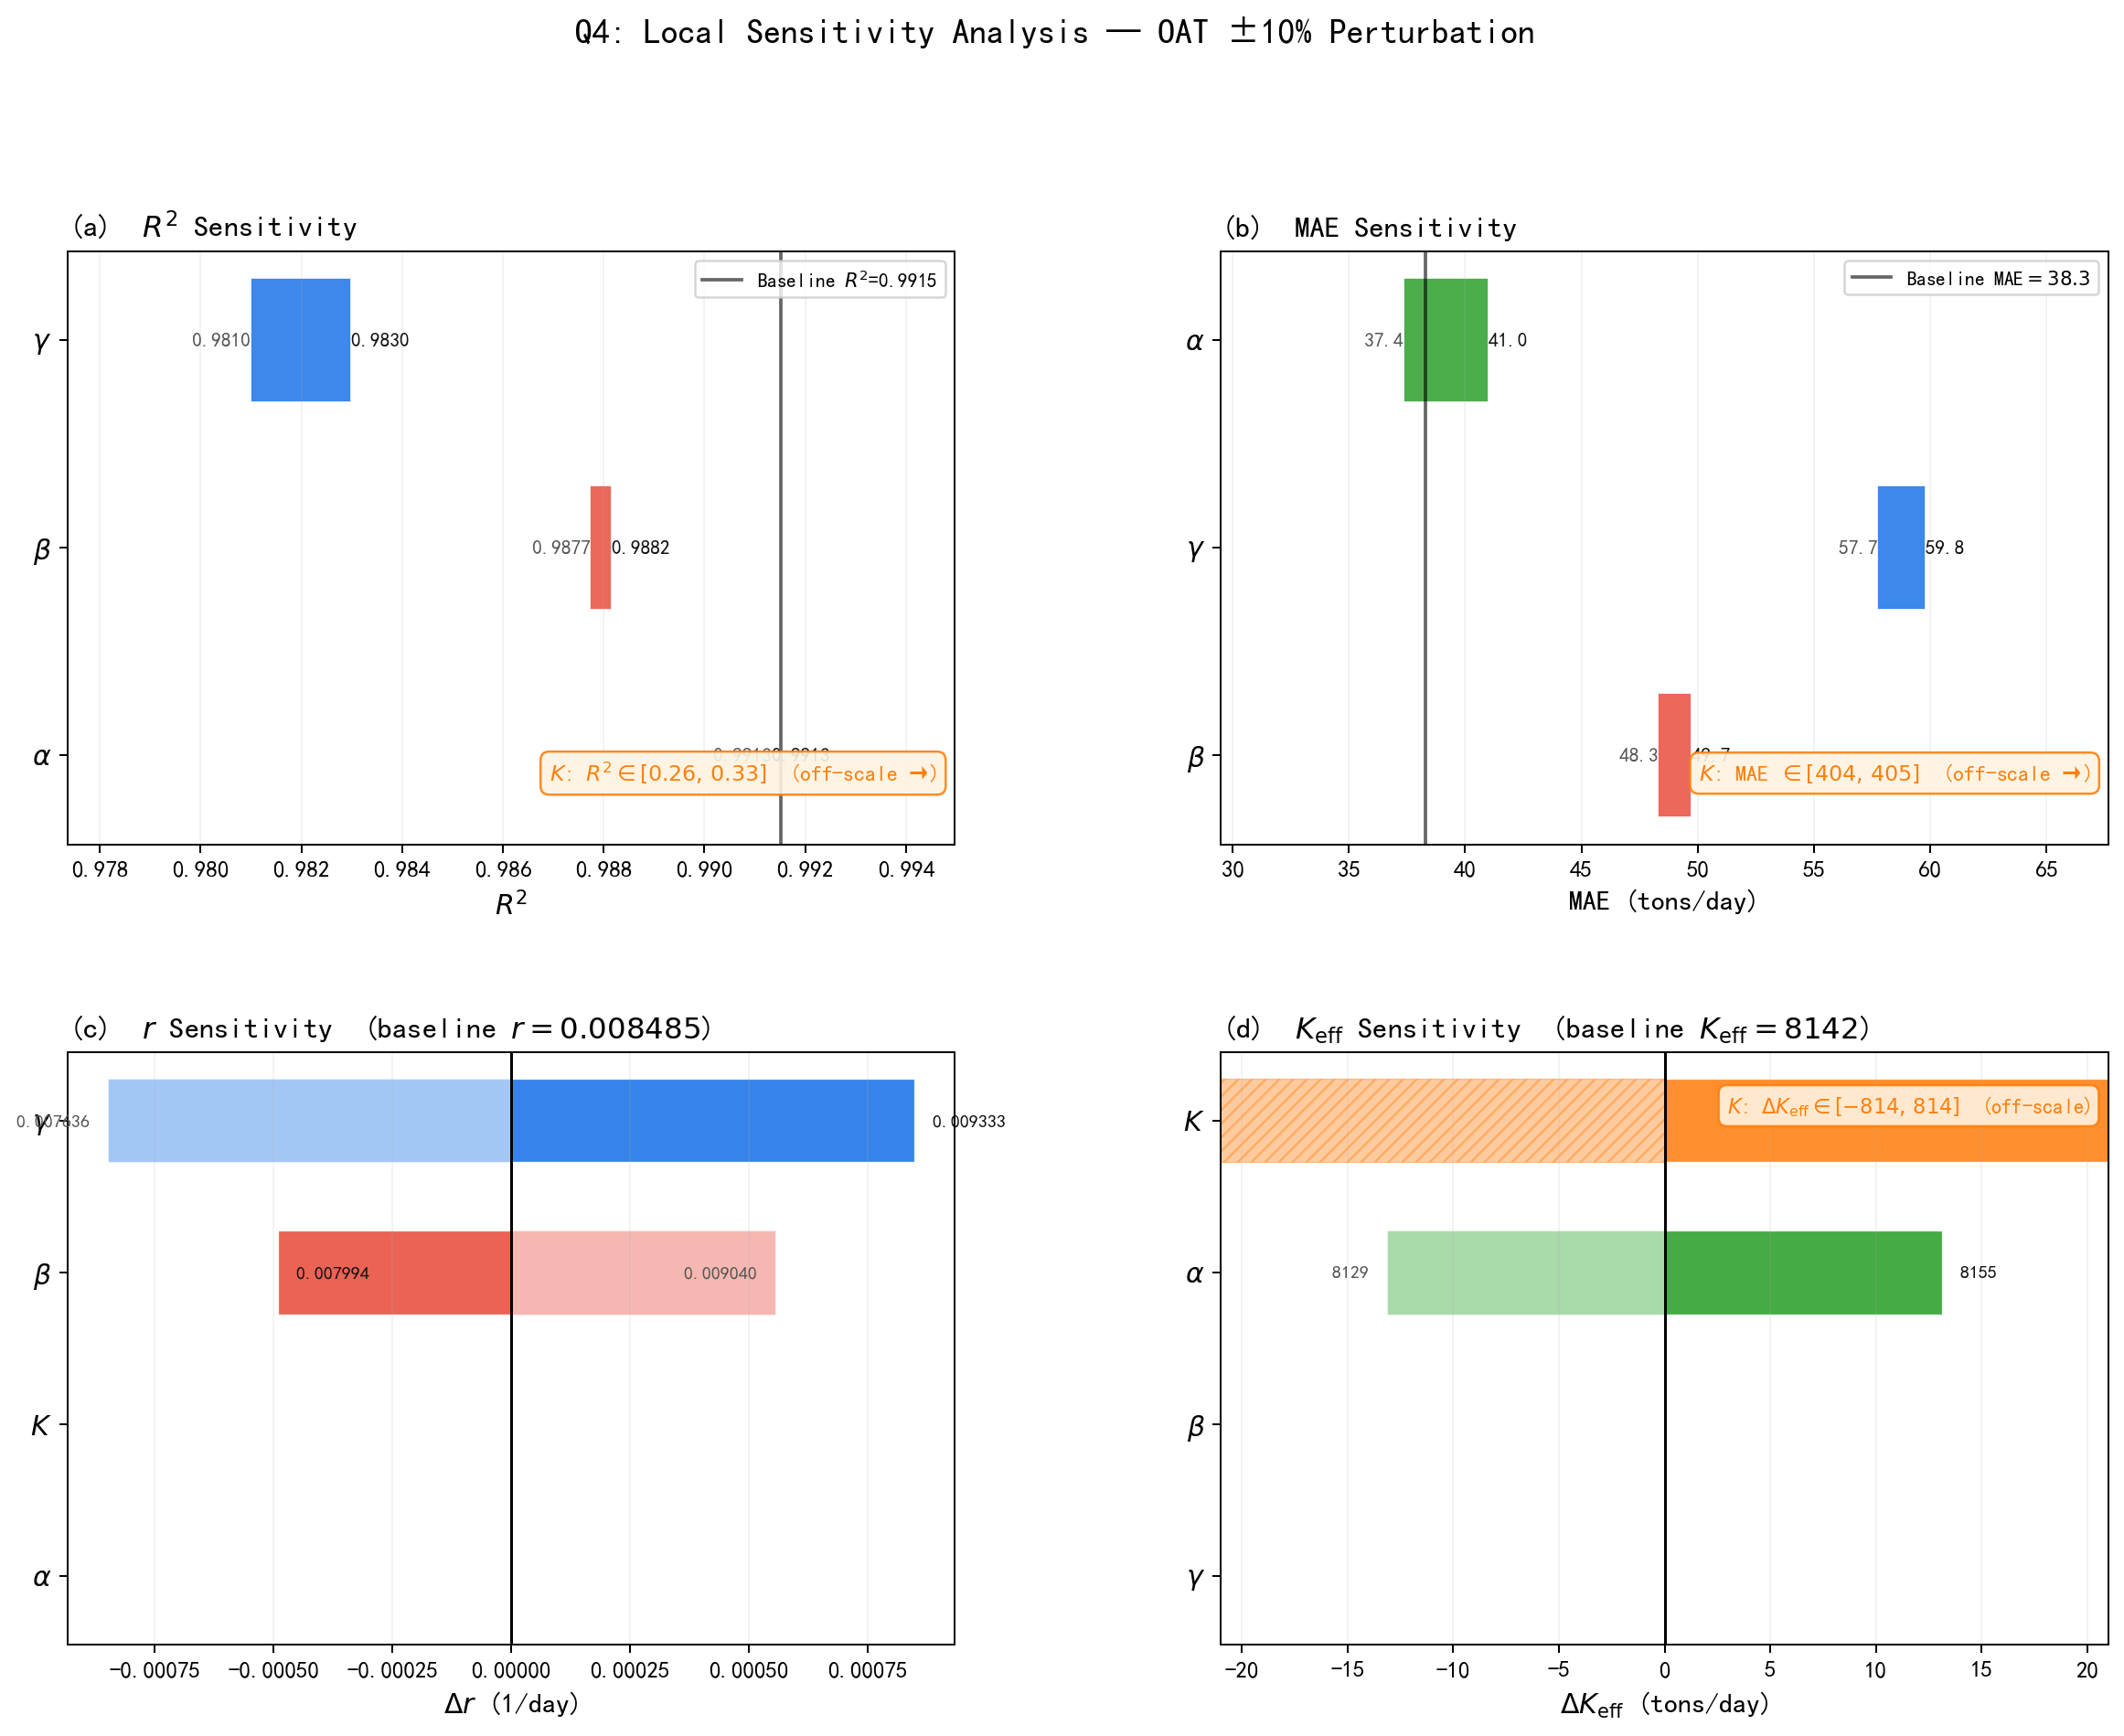
\includegraphics[width=\textwidth]{sensitivity_tornado.png}
\caption{龙卷风图：各参数 $\pm 10\%$ 对 $R^2$、MAE、$r$、$K_{\text{eff}}$ 的影响。
注意 (a)(b)(d) 中 $K$ 的影响远超坐标轴范围（以橙色文本框标注离轴数值），
意在让读者关注非 $K$ 参数之间的差异。}
\label{fig:tornado}
\end{figure}

\begin{figure}[htbp]
\centering
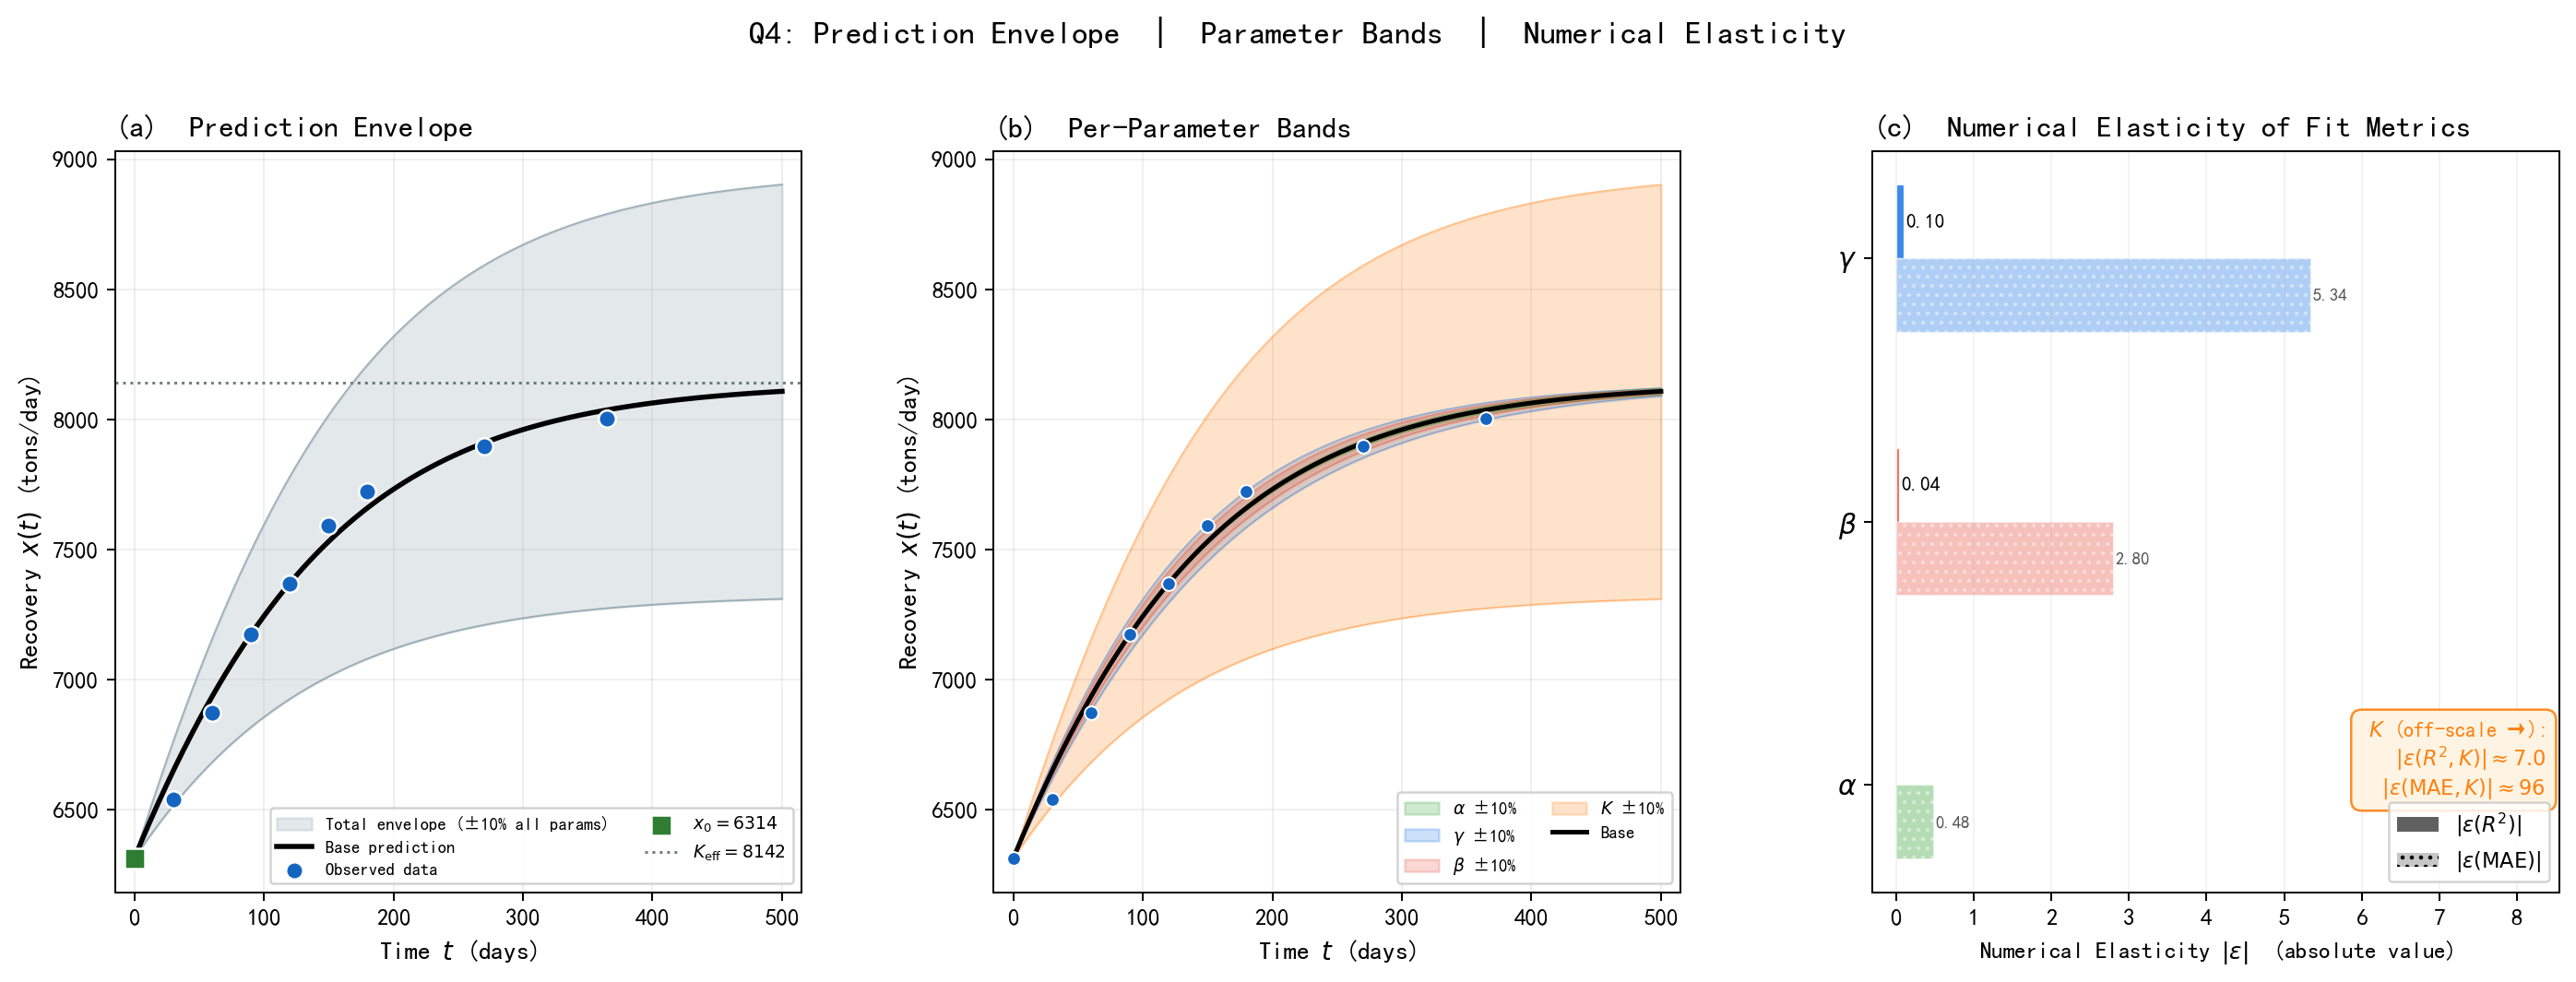
\includegraphics[width=\textwidth]{sensitivity_envelope.png}
\caption{(a) 所有参数 $\pm 10\%$ 的总预测包络线——包络宽度完全由 $K$ 主导；
(b) 各参数独立扰动带——$K$（橙色）的带宽远超其余参数；
(c) 拟合指标的数值弹性——$K$ 的弹性（$\sim 96$ for $R^2$）以文本框标注于右侧，已超出其余参数坐标范围约两个数量级。}
\label{fig:envelope}
\end{figure}

\subsection{与 Q3 稳定性结论的联合分析}

Q3 证明了系统在数学上具有结构稳定性——只要 $\alpha, \beta \geq 0$，
平衡点 $x^* = K_{\text{eff}}$ 恒为渐近稳定，不存在分岔。
然而，\textbf{结构稳定 $\neq$ 运营安全}。

Q4 灵敏度分析揭示了稳定性的\textbf{定量脆弱面}：

\begin{enumerate}
  \item \textbf{稳定性保证了方向，灵敏度决定了精度}：
        Q3 告诉我们 $x(t) \to K_{\text{eff}}$ 一定会发生；
        Q4 告诉我们，如果 $K$ 估计偏差 $10\%$，那么``一定会趋向的目标值''
        本身就是错的（$K_{\text{eff}}$ 偏差 $\sim 814$ 吨/天）。
        \textbf{系统会忠实趋向错误的目标}——这是另一种形式的``稳定性陷阱''。

  \item \textbf{恢复速度的安全边界}：
        Q3 定义了 $\beta \leq \gamma/r_{\min} - 1 = 3.40$（取 $r_{\min} = 0.005$）。
        当前 $\beta = 1.59$，裕度 $1.81$。
        Q4 进一步表明，在现有裕度内，$\beta$ 的敏感度不高——
        即使 $\beta$ 恶化 $10\%$（增至 $1.75$），$R^2$ 仍为 $0.9882$。
        \textbf{增长速度方面的安全裕度是充足的}——短期内不必担忧收敛过慢。

  \item \textbf{真正的风险不在数学分岔，而在参数误判}：
        Q3 的安全边界（$\beta < 3.40$）很宽，运营中几乎不可能触及。
        但 Q4 揭示：$K$ 的 $\pm 10\%$ 偏差就能让模型 $R^2$ 跌至 $0.3$。
        \textbf{回收体系最大的风险不是系统崩溃，而是对容量上限的误判导致的规划失误}——
        例如低估 $K$ 则规划产能不足（站点提前满溢、居民投递无门），
        高估 $K$ 则造成资源浪费（建设过多站点、运营成本高企）。
\end{enumerate}

\subsection{关键结论与长效调控策略}

基于 Q3 稳定性分析和 Q4 灵敏度分析的联合发现，
为``沪尚回收''体系的长效稳定运行提出以下定量策略建议：

\subsubsection*{1. 优先级一：精确测定基准容量 $K$（最高回报）}

$K$ 是模型的核心支柱——$\pm 10\%$ 偏差直接使 $R^2$ 从 $0.9915$ 崩塌至 $\sim 0.3$，
敏感度远超其他参数（$\times 30$--$170$）。然而 $K$ 恰恰是四个参数中\textbf{最难直接测量}的：
它涉及常住人口总量、人均可回收物产生系数、低价值品类占比、回收网络地理覆盖率等外生变量，
任何一个估计环节的偏差都会沿 $\varepsilon(K_{\text{eff}}, K) = 1$ 的比例关系
直接传导到模型预测。

\textbf{建议措施}：
\begin{itemize}
  \item 开展全市可回收物潜力普查（抽样调查 + 遥感人口密度估算），
        将 $K$ 的估计误差控制在 $\pm 5\%$ 以内——这可将 $R^2$ 损失限制在可接受范围。
  \item 每年更新 $K$ 的估计值（因人口流动、消费结构变化等因素会改变基准容量），
        将模型重新校准纳入年度运维计划。
\end{itemize}

\subsubsection*{2. 优先级二：精准降低抑制系数 $\beta$（最高效的调控杠杆）}

降低 $\beta$（改善运营效率）对恢复速度的影响是提升 $\alpha$（扩大促进）
对容量影响的 $\sim 38$ 倍（$0.6143 / 0.0161 \approx 38$）。
且题目背景中明确指出了三大抑制源头：

\begin{itemize}
  \item \textbf{清运不及时}（智能回收箱满溢后居民无法投递）：
        优化清运调度算法，基于满溢传感器实现动态路线规划，将平均清运延迟控制在阈值以下。
  \item \textbf{老年群体操作困难}（智能设备适配性不足）：
        增设人工辅助回收点与智能设备并行；开发语音交互、大字体简化界面等适老化改造；
        在老龄化程度高的社区保留或增加传统回收渠道。
  \item \textbf{低价值品类回收意愿低}（源头分类不精细）：
        试行低价值可回收物补贴机制（按重量阶梯补贴到社区或居民），
        降低居民对低价值品类的分类心理成本。
\end{itemize}

当前 $\beta$ 已使有效增长率降至固有水平的 $38.6\%$，
说明抑制效应远大于促进效应——\textbf{运营摩擦是当前回收体系的头号效率瓶颈}。
然而 Q4 也提示：$\beta$ 弹性为 $-0.61$，边际收益递减，
应将资源集中在消除\textbf{最严重的瓶颈环节}
（如清运延迟和适老化），而非追求面面俱到的微优化。

\subsubsection*{3. 优先级三：重新审视促进策略 $\alpha$ 的着力点（当前策略需转型）}

$\alpha$ 的弹性仅为 $0.016$——全市已建成 1.5 万个服务点 + 4300 台智能回收箱 + 800 个惠民服务点
后，站点数量增加对容量的边际贡献几乎为零。\textbf{但这并不意味着宣传引导没有价值}——
它可能通过以下渠道间接发挥作用：

\begin{itemize}
  \item \textbf{提升 $\gamma$}：宣传引导提高居民基础参与度，推升固有增长率，
        而非扩大饱和容量。应设计 AB 测试验证宣传投入对 $\gamma$ 的边际效应。
  \item \textbf{降低 $\beta$}：知识普及降低居民分类错误率（减少二次分拣的运维负担），
        社区动员提高居民对满溢和故障的主动上报率（间接改善清运效率）。
  \item \textbf{优化品类结构}：针对低价值品类的专项宣传可能改变 $K$ 的品类构成，
        而非 $K_{\text{eff}}$ 的总量。
\end{itemize}

\textbf{建议措施}：
\begin{itemize}
  \item 停止以``增加站点数量''为核心考核指标的扩张策略——
        当前覆盖率已接近饱和，边际回报极低。
  \item 将促进工作的考核重心从``建了多少点''转向``每个点服务了多少人、
        实际投递频次和居民满意度''——关注促进策略对 $\gamma$ 和 $\beta$ 的间接效应，
        而非 $\alpha$ 本身。
  \item 将释放出的资源（人力、资金、管理精力）重新分配到 $\beta$ 的降低上
        （清运优化、适老化改造），实现\textbf{从规模扩张向质量提升的战略转型}。
\end{itemize}

\subsubsection*{4. 优先级四：$\gamma$ 保持监测即可（低维护成本）}

$\gamma$ 的扰动影响中等（$R^2$ 保持在 $0.98$ 以上），弹性为 1（线性传递，无放大），
且 $\gamma$ 受制于居民回收习惯等慢变量，短期波动有限。
建议每季度通过小样本抽样调查验证 $\gamma$ 的稳定性，无需高频精确跟踪。

\subsubsection*{5. 总体资源分配建议}

综合 Q3 和 Q4 的全部量化证据，建议``沪尚回收''体系的长效运维资源按以下优先级分配：

\begin{center}
\begin{tabular}{clp{7cm}}
\toprule
优先级 & 参数 & 行动方向与预期效果 \\
\midrule
\textbf{1} & $K$（基准容量） &
  \textbf{精确测量}：开展潜力普查，将估计误差压缩至 $\pm 5\%$ 内。
  预期效果：确保模型预测的可靠性基础不被摧毁。 \\

\textbf{2} & $\beta$（抑制） &
  \textbf{定向削减}：优化清运调度 + 适老化改造 + 低价值品类补贴。
  预期效果：每降低 $\beta$ 约 $10\%$，有效增长率 $r$ 提升约 $6.5\%$。 \\

\textbf{3} & $\alpha$（促进） &
  \textbf{战略转型}：从扩大站点数量转向提升站点服务质量，
  考核指标从覆盖率转向人均使用频次和满意度。关注促进策略对 $\gamma$、$\beta$ 的间接效应。
  预期效果：释放无效扩张的沉没成本，将资源重新导向高回报领域。 \\

\textbf{4} & $\gamma$（固有增长率） &
  \textbf{常规监测}：季度抽样验证，无需精确跟踪。系统对 $\gamma$ 的偏差具有鲁棒性。
  预期效果：维持对居民参与度长期趋势的基本感知。 \\
\bottomrule
\end{tabular}
\end{center}

\subsubsection*{6. 最终总结}

``沪尚回收''体系在数学上是安全的（Q3），
在参数不确定性面前是脆弱的（Q4），
而脆弱性高度集中在唯一参数——基准容量 $K$。

\begin{center}
\fbox{%
\begin{minipage}{0.90\textwidth}
\centering
\textbf{核心战略：守住 $K$ 的精度，抓住 $\beta$ 的优化，转变 $\alpha$ 的定位。}\\[4pt]
\begin{itemize}
  \item {\color{red}\textbf{$K$}}：精确估计是模型的生命线——估计偏差 $10\%$，模型崩溃；
  \item {\color{blue}\textbf{$\beta$}}：定向削减是最有效的效率杠杆——$\times 38$ 倍于促进策略；
  \item {\color{green!60!black}\textbf{$\alpha$}}：饱和扩张已是过去式——从``广铺网络''转向``精耕运营''；
  \item {\color{gray}\textbf{$\gamma$}}：保持感知即可——系统对此足够鲁棒。
\end{itemize}
\end{minipage}}
\end{center}

\subsubsection{模型评价}

\subsubsection{模型优点}

\begin{enumerate}
    \item 建模思路递进清晰，能够逐步反映回收体系从自然增长到复杂运营机制的演化过程；
    \item 参数具有明确实际意义，便于与回收体系的管理措施相对应；
    \item 同时考虑了增长规律、稳定性和灵敏度，能够为长期运维提供综合决策依据。
\end{enumerate}

\subsubsection{模型不足}

\begin{enumerate}
    \item 促进作用与抑制作用被视为阶段内恒定，未考虑其随时间变化的情况；
    \item 未进一步区分不同类型可回收物之间的差异；
    \item 模型基于全市总体数据，未体现区域间的空间异质性。
\end{enumerate}

\section{结论}

本文以“沪尚回收”体系为研究对象，围绕可回收物回收量的动态预测与回收体系稳定性分析，建立了递进式动力学建模框架。

首先，在仅考虑自然增长与容量约束的条件下，建立基础 Logistic 模型，用于描述回收量由初始水平逐渐增长并最终趋于饱和的基本规律。随后，引入促进系数 $\\alpha$ 与抑制系数 $\\beta$，结合题目给出的实测时序数据进行参数拟合，使模型能够同时反映宣传推广、站点完善等正向作用以及清运延迟、运维不足等负向作用，从而更真实地描述回收体系的动态演化过程。

在稳定性分析中，通过对模型平衡点的讨论，明确了系统存在稳定运行状态，并进一步给出了促进系数与抑制系数的合理取值区间，可用于划定回收体系稳定运行的安全边界和提前识别潜在失衡风险。

在灵敏度分析中，比较了固有增长率、促进系数、抑制系数以及潜在饱和总量的影响程度，结果表明，不同参数对系统稳定性和长期回收水平的影响存在明显差异，因此在实际运维中应优先关注对系统影响更显著的关键参数。

综合来看，本文建立的模型能够较好地刻画“沪尚回收”体系的增长、饱和与稳定运行特征，并为城市绿色回收体系的长期优化提供了定量分析框架。研究表明，保持充足的系统容量、降低运维与清运带来的抑制作用、并持续提升居民参与度，是实现城市绿色回收体系长效稳定运行的重要方向。

\begin{thebibliography}{99}

\bibitem{1} 西交利物浦大学数学建模训练 2026 Problem A 题目及附件数据.

\end{thebibliography}

\end{document}